\section{Internal Block Diagram - MCS}
As with the Battery Management System, the Motor Control System (MCS) is too complex to be represented propely on a IBD along with the rest of the systems. The complexity has instead been visualized on a seperate Internal Block Diagram. The result is seen below.
\fxnote{Opdater med HornOn + signalbeskrivelse - JOnathan}
\begin{figure}[H]
	\centering
	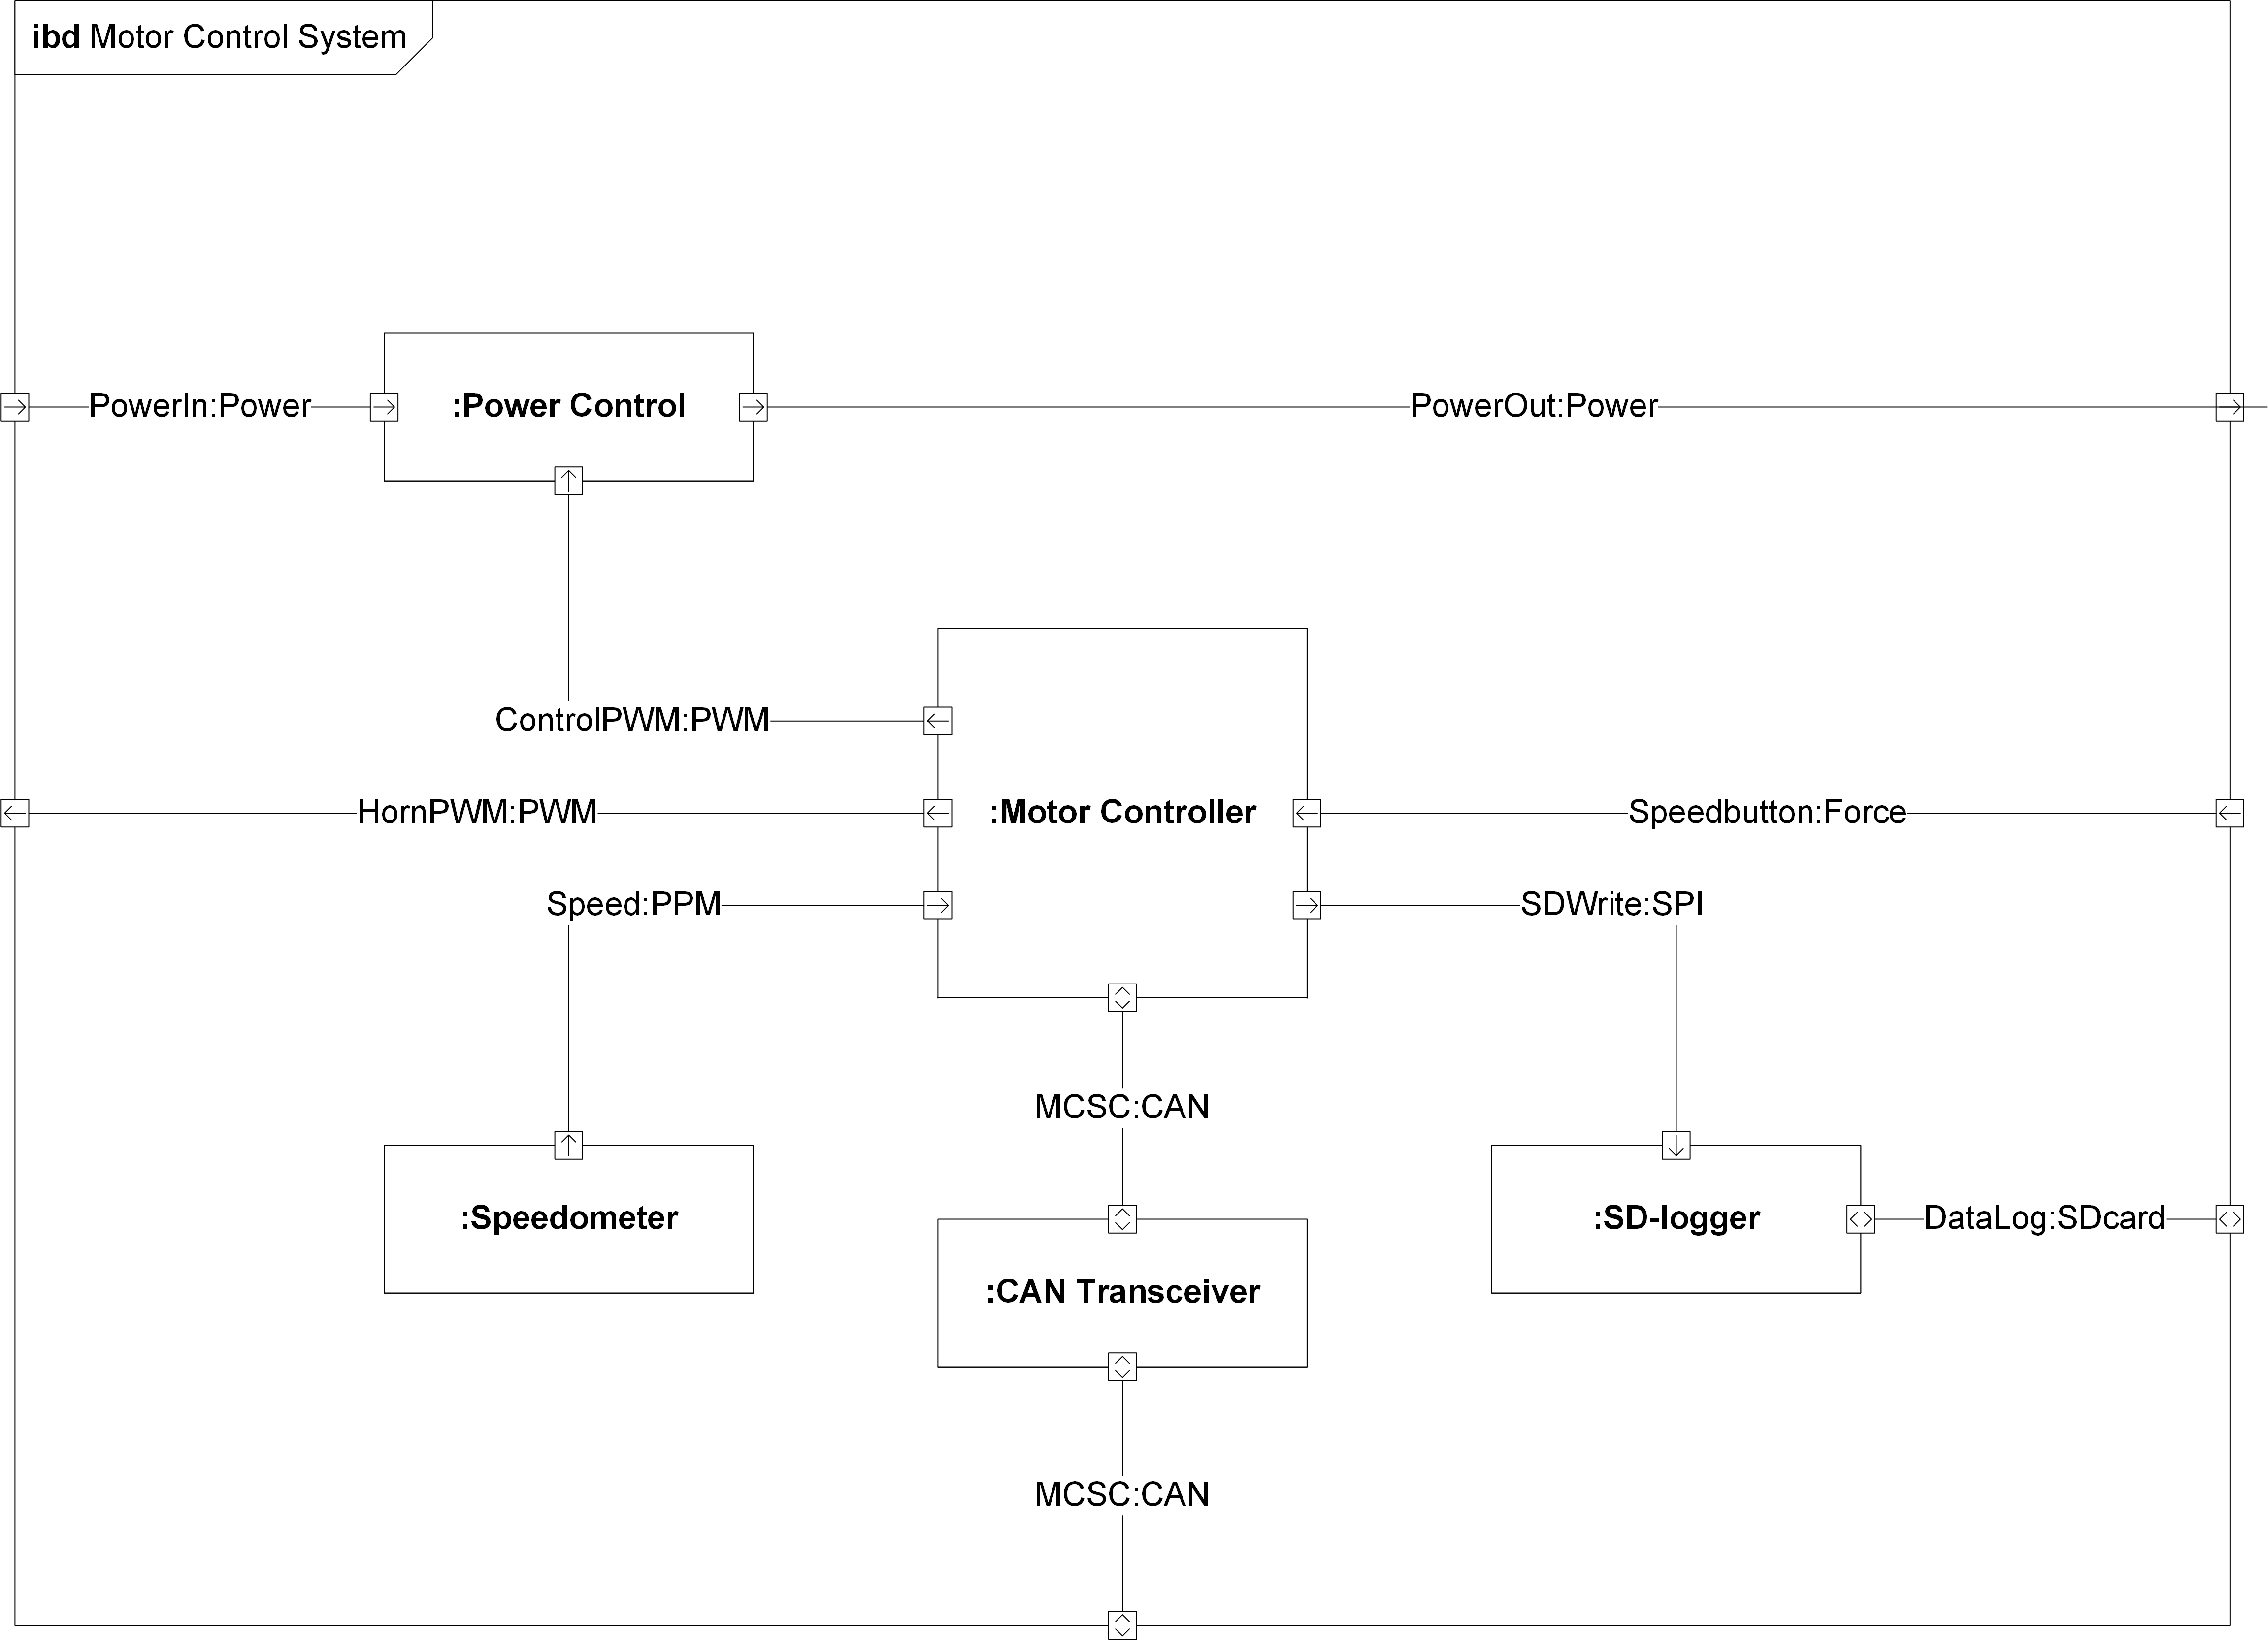
\includegraphics[width=1\linewidth]{Architecture/Diagrams/IBD_MCS}
	\caption{IBD for AU2's Motor Control System}
	\label{fig:IBD_MCS}
\end{figure}

It should be noted that each of the blocks in the MCS is connected with the signal called 'SupplyMCS:Voltage' which supplies every block in MCS with 5 V. This signal has been omitted from the IBD to increase the simplicity.

\section{Signal description - MCS}
The signals and protocols used to communicate between the blocks in MCS are specified in this section.

\textbf{Block :MCS}\\
Block interface description:
\begin{itemize}
	\item \textbf{SupplyMCS:Voltage}\\
	Direction: [External] $\rightarrow$ [Every Block]\\
	Description: Power supply to the systems.
	\item \textbf{HornPWM:PWM}\\
	Direction: [x] $\rightarrow$ [y]\\
	Description:
	\item \textbf{PowerIn:Power}\\
	Direction: [x] $\rightarrow$ [y]\\
	Description:
	\item \textbf{PowerMeas:Power}\\
	Direction: [x] $\rightarrow$ [y]\\
	Description:
	\item \textbf{PowerOut:Power}\\
	Direction: [x] $\rightarrow$ [y]\\
	Description:
	\item \textbf{MCSC:CAN}\\
	Direction: [x] $\rightarrow$ [y]\\
	Description:
\end{itemize}

\textbf{Block :Power Control}\\
Block interface description:
\begin{itemize}
	\item \textbf{SupplyMCS:Voltage}\\
	Direction: [External] $\rightarrow$ [Power Control]\\
	Description: Power supply to the block.
	\item \textbf{}\\
	Direction: [x] $\rightarrow$ [y]\\
	Description:
\end{itemize}

\textbf{Block :Joulemeter}\\
Block interface description:
\begin{itemize}
	\item \textbf{SupplyMCS:Voltage}\\
	Direction: [External] $\rightarrow$ [Joulemeter]\\
	Description: Power supply to the block.
	\item \textbf{}\\
	Direction: [x] $\rightarrow$ [y]\\
	Description:
\end{itemize}

\textbf{Block :Motor Controller}\\
Block interface description:
\begin{itemize}
	\item \textbf{SupplyMCS:Voltage}\\
	Direction: [External] $\rightarrow$ [Motor Controller]\\
	Description: Power supply to the block.
	\item \textbf{}\\
	Direction: [x] $\rightarrow$ [y]\\
	Description:
\end{itemize}

\textbf{Block :Speedometer}\\
Block interface description:
\begin{itemize}
	\item \textbf{SupplyMCS:Voltage}\\
	Direction: [External] $\rightarrow$ [Speedometer]\\
	Description: Power supply to the block.
	\item \textbf{}\\
	Direction: [x] $\rightarrow$ [y]\\
	Description:
\end{itemize}

\textbf{Block :CAN Tranceiver}\\
Block interface description:
\begin{itemize}
	\item \textbf{SupplyMCS:Voltage}\\
	Direction: [External] $\rightarrow$ [CAN Tranceiver]\\
	Description: Power supply to the block.
	\item \textbf{µCan:}\\
	Direction: [Motor Controller] $\leftrightarrow$ [Can Tranceiver]\\
	Description:
	\item \textbf{MCSC:CAN}\\
	Direction: [Can Tranceiver] $\leftrightarrow$ [External]\\
	Description:
\end{itemize}

\textbf{Block :SD-logger}\\
Block interface description:
\begin{itemize}
	\item \textbf{SupplyMCS:Voltage}\\
	Direction: [External] $\rightarrow$ [SD-logger]\\
	Description: Power supply to the block.
\end{itemize}